

\documentclass{article}


\usepackage{amssymb,amsmath,mathtools,xcolor,graphicx,xspace,colortbl,ragged2e,rotating} % 
\usepackage{amsfonts}  %% 010
\usepackage{amsmath}  %% 010
\usepackage{boxedminipage}  %% 100
\usepackage{graphics}  %% 100
\usepackage{ragged2e}  %% 100
\usepackage{wrapfig}  %% 100
\usepackage{xcolor}  %% 200
\graphicspath{{images/}}
\DeclareGraphicsExtensions{.pdf,.eps,.ps,.png,.jpg,.jpeg}
\begin{document}
\title{AI1110 Assignment 1
}
\author{
Dondapati Chandrahas Reddy
\\
AI21BTECH11010
}
\maketitle





\section{Question 3 (a)
}
{\Large Question:}



\begin{center}
\setlength\fboxrule{0in}\setlength\fboxsep{0.1in}\fcolorbox[HTML]{FFFFFF}{FFFFFF}{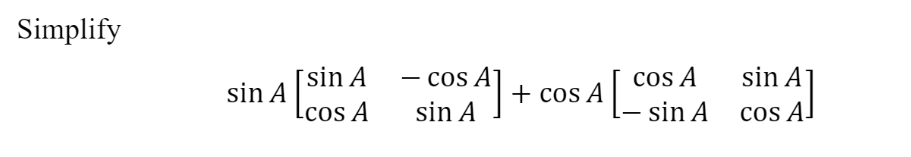
\includegraphics[ width=5.8125in, height=1in,]{img1}
}
\end{center}
{\Large Solution:
\newline }


Performing scalar multiplication we get



\begin{center}$\left [\begin{array}{cc}\sin ^{2}A &  -\sin A\cos A \\
\sin A\cos A & \sin ^{2}A\end{array}\right ] +\left [\begin{array}{cc}\cos ^{2}A & \cos A\sin A \\
 -\cos A\sin A & \cos ^{2}A\end{array}\right ]$\newline \end{center}\par
Adding the matrices



\begin{center}$\left [\begin{array}{cc}\sin ^{2}A +\cos ^{2}A &  -\sin A\cos A +\cos A\sin A \\
\sin A\cos A -\cos A\sin A & \sin ^{2}A +\cos ^{2}A\end{array}\right ]$\linebreak\relax \end{center}\par
Simplifying the expressions we get



\begin{center}$\left [\begin{array}{cc}1 & 0 \\
0 & 1\end{array}\right ]$\end{center}\par
\end{document}